\documentclass[runningheads]{llncs}

\usepackage[T1]{fontenc}
\usepackage{graphicx}
\usepackage{hyperref}

\begin{document}

\title{IMDb Data Engineering Pipeline}

\author{Savin Mihai-Alexandru \\ \vspace{0.1cm} \normalsize{August 24, 2026}}
\institute{}

\maketitle

\section{Executive Summary}
This project implements an automated, end-to-end data engineering pipeline that extracts raw IMDb datasets, loads them into a DuckDB data warehouse, and transforms them into a query-ready star schema using dbt. Orchestrated by Apache Airflow, the pipeline ultimately answers complex analytical questions regarding top-rated directors, movie runtime evolution, and the ratio of hidden gems to overrated titles within various cinematic genres.

\section{Dataset Description}
The primary data source consists of bulk exports from the official IMDb website, accessible via \url{datasets.imdbws.com}.

\begin{itemize}
    \item \textbf{Source, Size, and Frequency:} The dataset contains millions of rows distributed across seven large, compressed TSV files, which IMDb updates on a daily basis.
    \item \textbf{Scoping Decisions:} The extraction process retrieves all seven core files provided by the platform (\texttt{name.basics}, \texttt{title.akas}, \texttt{title.basics}, \texttt{title.crew}, \texttt{title.episode}, \texttt{title.principals}, and \texttt{title.ratings}) to ensure a complete foundation for the data warehouse before any targeted transformations occur.
\end{itemize}

\subsection{Raw Data Structure}
Before being processed and cleaned in dbt, the original non-commercial dataset operates on a relational structure centered around two main pillars: \textbf{Productions} (identified by the \texttt{tconst} primary key) and \textbf{Persons} (identified by the \texttt{nconst} primary key).

The Productions pillar includes tables such as \texttt{title.basics} (core movie and show metadata), \texttt{title.akas} (regional alternative titles), \texttt{title.ratings} (user scores and votes), and \texttt{title.episode} (TV series hierarchy). The Persons pillar is anchored by \texttt{name.basics}, which contains biographical data for actors, directors, and crew members.

These two domains are closely linked via intersection bridge tables, notably \texttt{title.crew} (providing preliminary director and writer lists) and \texttt{title.principals} (detailing the exact cast and crew billing, including character names).

Figure \ref{fig:og_diagram} illustrates the Entity-Relationship Diagram of this raw dataset prior to its dimensional modeling.

\begin{figure}[h!]
\centering

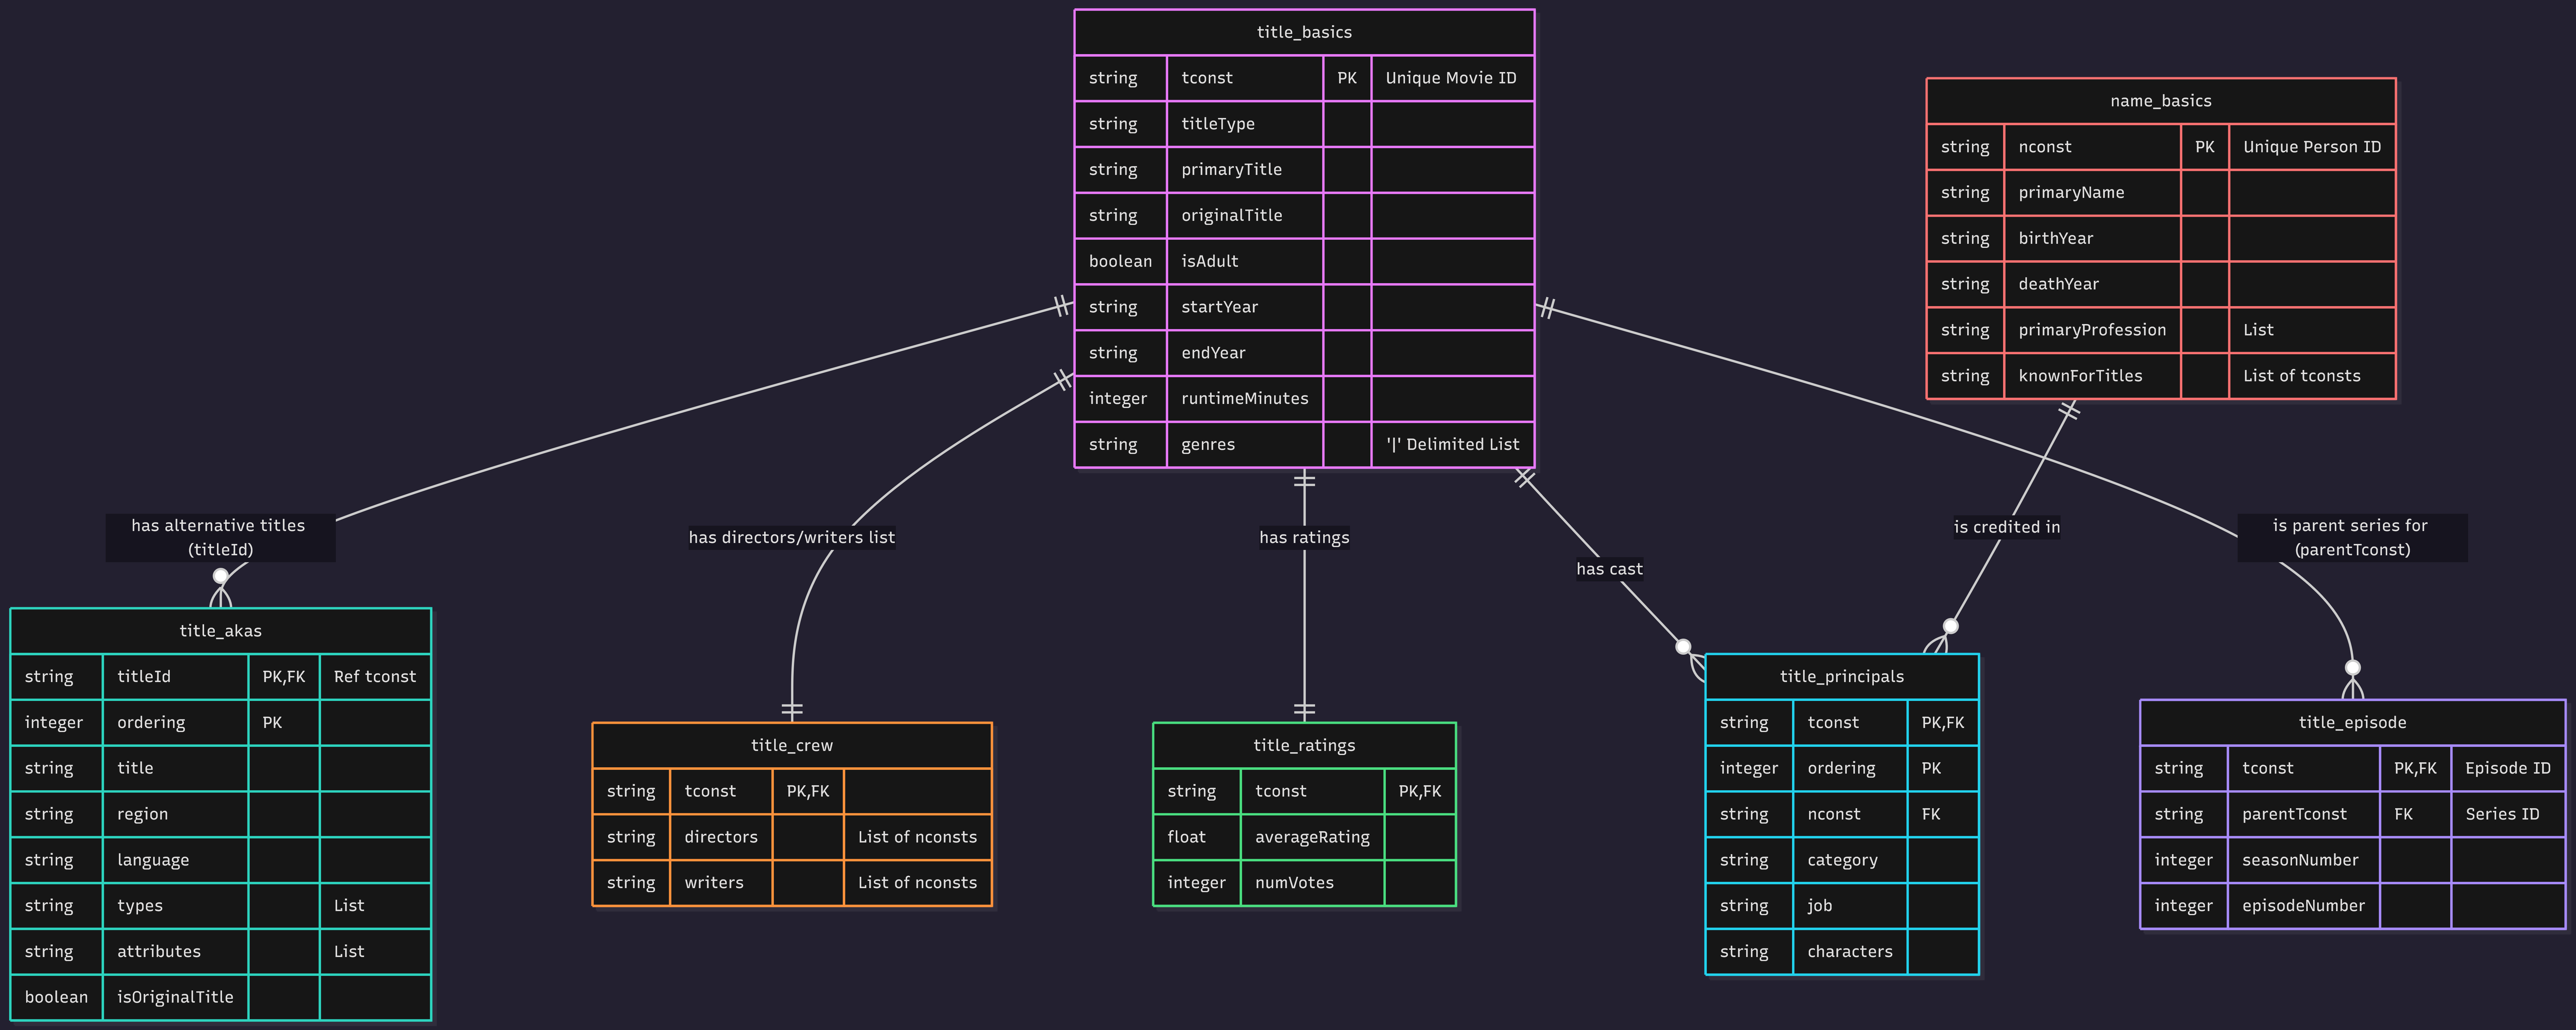
\includegraphics[width=0.9\textwidth]{og_diagram.png}
\caption{Entity-Relationship Diagram of the raw IMDb dataset}
\label{fig:og_diagram}
\end{figure}

To better understand the extraction and loading phases, the raw tables are detailed below based on their specific domains:

\subsubsection*{The Productions Pillar}
\begin{itemize}
    \item \textbf{\texttt{title.basics}:} The core table for all productions. It includes the unique identifier (\texttt{tconst}), format (\texttt{titleType}), release names, runtime, and a delimited list of genres.
    \item \textbf{\texttt{title.akas}:} Stores alternative regional titles and translations, linking back to the main movie via \texttt{titleId}. It includes localization details such as region and language.
    \item \textbf{\texttt{title.ratings}:} The table storing user scores, containing the movie ID, the average score (\texttt{averageRating}), and the total number of votes.
    \item \textbf{\texttt{title.episode}:} Used to map specific TV episodes (\texttt{tconst}) to their parent series (\texttt{parentTconst}), alongside season and episode numbers.
\end{itemize}

\subsubsection*{The Persons Pillar}
\begin{itemize}
    \item \textbf{\texttt{name.basics}:} The foundational table for industry personnel. It holds the unique person identifier (\texttt{nconst}), credited name, birth/death years, primary professions, and a denormalized list of titles they are known for.
\end{itemize}

\subsubsection*{Intersection (Bridge) Tables}
\begin{itemize}
    \item \textbf{\texttt{title.crew}:} A preliminary relational link providing a comma-separated list of director and writer IDs for a specific title.
    \item \textbf{\texttt{title.principals}:} A highly detailed bridge table outlining the exact roles individuals had in a production. It links \texttt{tconst} and \texttt{nconst}, specifying the billing order, role category (e.g., actor, director), and a JSON array of character names played.
\end{itemize}

\section{Architecture Overview}
The project's architecture integrates three main technologies, operating on a scheduled basis to ensure data freshness:

\begin{itemize}
    \item \textbf{Apache Airflow (Orchestrator):} Acts as the central scheduler and trigger mechanism. The DAG is designed to run sequentially, ensuring dependencies are strictly respected.
    \item \textbf{DuckDB (Data Warehouse) \& Python:} A Python script, triggered by Airflow, handles the extraction of the raw \texttt{.tsv.gz} files. To optimize storage and query performance, these files are first converted into Parquet format. Only the resulting Parquet files are then loaded into the DuckDB database as raw tables.
    \item \textbf{dbt (Transformer):} Once the data lands in DuckDB, Airflow triggers dbt to execute the data modeling phases. dbt handles type casting, filtering, table joins, data testing, and snapshotting, ultimately constructing the final query-ready star schema.
\end{itemize}

\section{Data Modeling Explanation}
To meet the analytical requirements of the project, the highly denormalized raw data was transformed into a robust star schema using dbt. This dimensional architecture optimizes query performance, resolves complex many-to-many relationships, and ensures accurate metric aggregations.

\subsection{Fact Table and Grain}
The core of the model is the \textbf{\texttt{fct\_title\_ratings}} table.
\begin{itemize}
    \item \textbf{Grain:} The grain is strictly defined as \textit{one row per title} (uniquely identified by \texttt{title\_id} / \texttt{tconst}).
    \item \textbf{Justification for Grain:} This explicit grain is critical because movie titles inherently have many-to-many relationships with both genres and industry personnel. If these relationships were flattened directly into the fact table, the row count would explode, leading to duplicated metrics and inaccurate statistical aggregations (e.g., counting a single movie's votes multiple times for every actor in it). The fact table isolates purely quantitative metrics: \texttt{average\_rating} and \texttt{num\_votes}.
\end{itemize}

\subsection{Dimension Tables}
The dimension tables provide the descriptive context necessary for filtering and grouping the facts:
\begin{itemize}
    \item \textbf{\texttt{dim\_title\_snapshot} (SCD Type 2):} This dimension tracks historical changes in core movie metadata. IMDb periodically corrects or reclassifies attributes such as \texttt{runtime\_minutes} or \texttt{genres}. By implementing a Slowly Changing Dimension (SCD Type 2) via dbt snapshots, the model generates surrogate keys (\texttt{dbt\_scd\_id}) and tracking timestamps (\texttt{dbt\_valid\_from}, \texttt{dbt\_valid\_to}, \texttt{is\_active}). This preserves historical metadata states as they were at the time of each load, rather than silently overwriting them.
    \item \textbf{\texttt{dim\_person}:} The central dimension for industry personnel, built by exploding the denormalized \texttt{knownForTitles} array from the raw data. It stores the \texttt{primary\_name} and \texttt{birth\_year}.
    \item \textbf{\texttt{dim\_year} \& \texttt{dim\_genre}:} Helper dimensions used to accelerate global aggregations, such as grouping movie runtimes by decade or normalizing genre names for comparative analysis.
\end{itemize}

\subsection{Bridge Tables (Resolving Many-to-Many Relationships)}
To maintain the strict one-row-per-title grain in the fact table while supporting complex filtering by cast or category, the schema implements two intersection (bridge) tables:
\begin{itemize}
    \item \textbf{\texttt{bridge\_title\_genres}:} Splits the original pipe-delimited genre strings into a normalized mapping between titles and individual genre IDs.
    \item \textbf{\texttt{bridge\_title\_crew}:} Unifies the raw \texttt{title.crew} and \texttt{title.principals} files into a single, cohesive table. It links a title (\texttt{title\_id}) to a person (\texttt{name\_id}) and explicitly defines their \texttt{role} (e.g., director, actor, writer).
\end{itemize}

Figure \ref{fig:erd_star} illustrates the final Star Schema design, demonstrating how the central fact table connects to the surrounding dimensions and bridge tables.

\begin{figure}[h!]
\centering
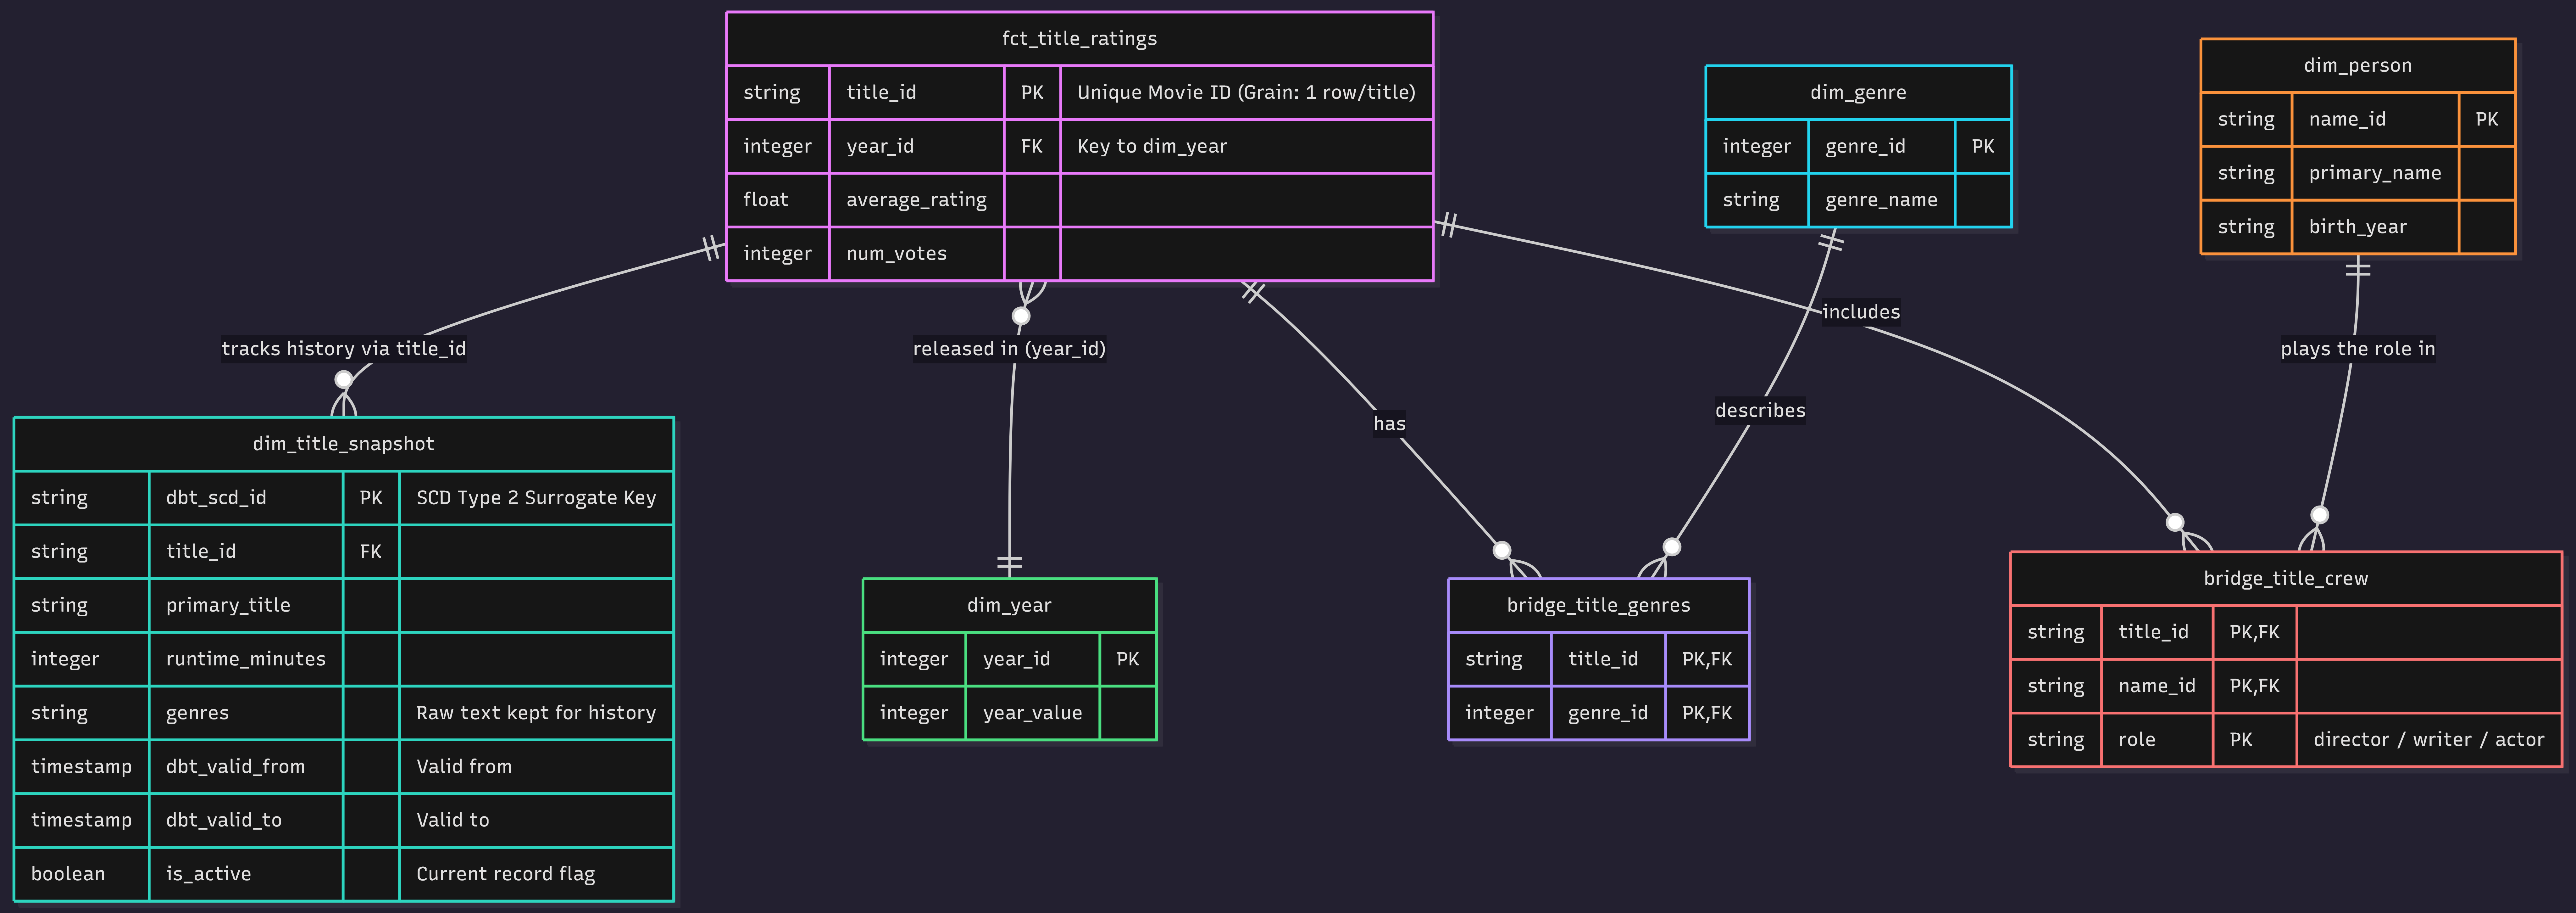
\includegraphics[width=0.9\textwidth]{erd_star.png}
\caption{Entity-Relationship Diagram of the finalized IMDb Star Schema}
\label{fig:erd_star}
\end{figure}

\section{Project Structure Walkthrough}
The repository is organized to separate orchestration, ingestion, transformation, and analytical outputs cleanly. Below is a walkthrough of the folder layout and the purpose of each directory:

\section{Project Structure Walkthrough}
The repository is organized to separate orchestration, ingestion, transformation, and analytical outputs cleanly. Below is a walkthrough of the folder layout and the purpose of each directory:

\begin{itemize}
    \item \textbf{\texttt{airflow/}} - Contains Apache Airflow orchestration files, including the DAG definitions (\texttt{dags/}) and Python dependencies (\texttt{requirements.txt}), to manage pipeline execution.
    \item \textbf{\texttt{analyses/}} - Stores the final business analytical SQL queries used to answer the project's core deliverable questions.
    \item \textbf{\texttt{data/}} - Acts as the landing directory for the raw IMDb datasets (\texttt{.tsv.gz} files) prior to their extraction and ingestion.
    \item \textbf{\texttt{dbt\_packages/}} - Contains external dbt packages downloaded as dependencies for the data transformation models.
    \item \textbf{\texttt{logs/}} - Stores execution logs for Airflow tasks and the overall data pipeline, essential for troubleshooting failures.
    \item \textbf{\texttt{macros/}} - Houses reusable dbt macros for custom SQL functions (e.g., extracting decades) and custom testing logic (\texttt{tests/}) to keep the codebase DRY (Don't Repeat Yourself).
    \item \textbf{\texttt{models/}} - The core dbt transformation folder, sequentially structured into \texttt{staging/} (cleaning, casting, and null handling), \texttt{intermediate/} (data reshaping steps, such as unnesting arrays, required before dimensional modeling), and \texttt{marts/} (the final query-ready Fact and Dimension tables).
    \item \textbf{\texttt{scripts/}} - Holds Python utility scripts, such as \texttt{load\_imdb.py} for DuckDB ingestion and \texttt{generate\_charts.py} for producing analytical visualizations.
    \item \textbf{\texttt{seeds/}} - Contains dbt seed files, which are static mapping CSVs loaded directly into the database as reference tables.
    \item \textbf{\texttt{snapshots/}} - Houses dbt snapshot definitions used to implement SCD Type 2 tracking for slowly changing dimensions (e.g., \texttt{dim\_title\_snapshot}).
    \item \textbf{\texttt{tests/}} - Stores custom dbt data tests to ensure data quality, referential integrity, and business rule enforcement across the pipeline.
    \item \textbf{\texttt{visualizations/}} - The output directory for the auto-generated analytical plots (\texttt{.png} files) created by the Python charting script.
    \item \textbf{\texttt{warehouse/}} - The destination folder for the compiled local \texttt{imdb.duckdb} database file, acting as the analytical data warehouse.
    \item \textbf{\texttt{.env / .env.example}} - Configuration files used for securely managing environment variables required by Docker and Airflow.
    \item \textbf{\texttt{db\_original.md / db\_star.md}} - Markdown documentation detailing the schema definitions of the raw IMDb data and the final Star Schema design.
\end{itemize}

\section{Airflow DAG Explanation}

The pipeline is orchestrated by Apache Airflow via a Directed Acyclic Graph (DAG) named \texttt{imdb\_pipeline}.

\subsection{Schedule and Configuration}
The DAG is configured to run on a \texttt{@daily} schedule, ensuring the data warehouse stays synchronized with IMDb's daily updates. To ensure fault tolerance and meet operational standards, the DAG configuration includes a default retry policy of one attempt (\texttt{retries: 1}) with a one-minute delay upon task failure.

\subsection{Task Dependencies and Execution Flow}
The pipeline executes sequentially, strictly enforcing dependencies to ensure data integrity before proceeding to the next logical stage. Figure \ref{fig:dag_view} displays the Graph View of the DAG from the Airflow UI.

\begin{figure}[h!]
\centering

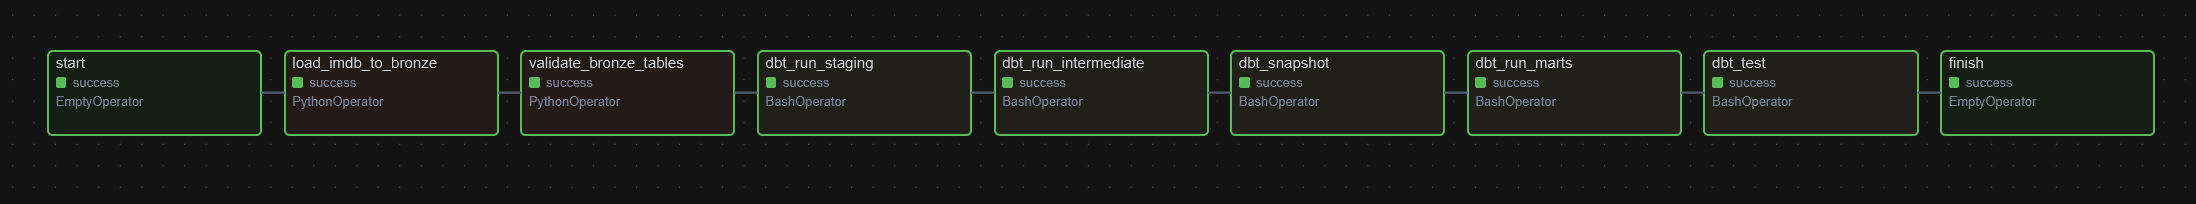
\includegraphics[width=0.9\textwidth]{dag_graph_view.png}
\caption{Airflow Graph View illustrating the sequential execution flow of the IMDb pipeline}
\label{fig:dag_view}
\end{figure}

The logical stages and their respective tasks are defined as follows:

\begin{enumerate}
    \item \textbf{\texttt{start} (EmptyOperator):} A dummy task marking the beginning of the DAG execution.
    \item \textbf{\texttt{load\_imdb\_to\_bronze} (PythonOperator):} Handles the Extraction and Loading phase. It reads the raw TSV files, converts them into Parquet format for optimized storage, and loads them directly into DuckDB's \texttt{bronze} schema.
    \item \textbf{\texttt{validate\_bronze\_tables} (PythonOperator):} A preliminary validation step designed to fail fast. It verifies that the DuckDB bronze tables were successfully populated and are not empty before beginning resource-intensive transformations.
    \item \textbf{\texttt{dbt\_run\_staging} (BashOperator):} Initiates the dbt transformation phase by running models in the \texttt{staging/} directory, handling column renaming, type casting, and null handling.
    \item \textbf{\texttt{dbt\_run\_intermediate} (BashOperator):} Executes the models in the \texttt{intermediate/} directory, which apply necessary data reshaping logic (such as unnesting arrays) to prepare the data for dimensional modeling.
    \item \textbf{\texttt{dbt\_snapshot} (BashOperator):} Runs the dbt snapshot process to capture Slowly Changing Dimension (SCD Type 2) modifications on the \texttt{dim\_title} metadata.
    \item \textbf{\texttt{dbt\_run\_marts} (BashOperator):} Executes the final dimensional models in the \texttt{marts/} directory, joining dimensions and facts into the final query-ready star schema.
    \item \textbf{\texttt{dbt\_test} (BashOperator):} The final validation phase. It runs all generic schema tests (e.g., uniqueness, non-null) and custom data tests across the dbt project to guarantee data quality and referential integrity.
    \item \textbf{\texttt{finish} (EmptyOperator):} A dummy task signaling the successful completion of the pipeline.
\end{enumerate}

The execution sequence is strictly linear: \texttt{start} $\rightarrow$ \texttt{load} $\rightarrow$ \texttt{validate} $\rightarrow$ \texttt{staging} $\rightarrow$ \texttt{intermediate} $\rightarrow$ \texttt{snapshot} $\rightarrow$ \texttt{marts} $\rightarrow$ \texttt{test} $\rightarrow$ \texttt{finish}.

\section{dbt Lineage and Tests}

\subsection{Data Lineage}
The dbt lineage graph provides a visual representation of the data flow, illustrating the dependencies from the raw DuckDB \texttt{bronze} tables through the \texttt{staging} and \texttt{intermediate} layers, culminating in the final \texttt{marts} dimensional models. Figure \ref{fig:dbt_lineage} shows the full Directed Acyclic Graph (DAG) of the dbt project.

\begin{figure}[h!]
\centering

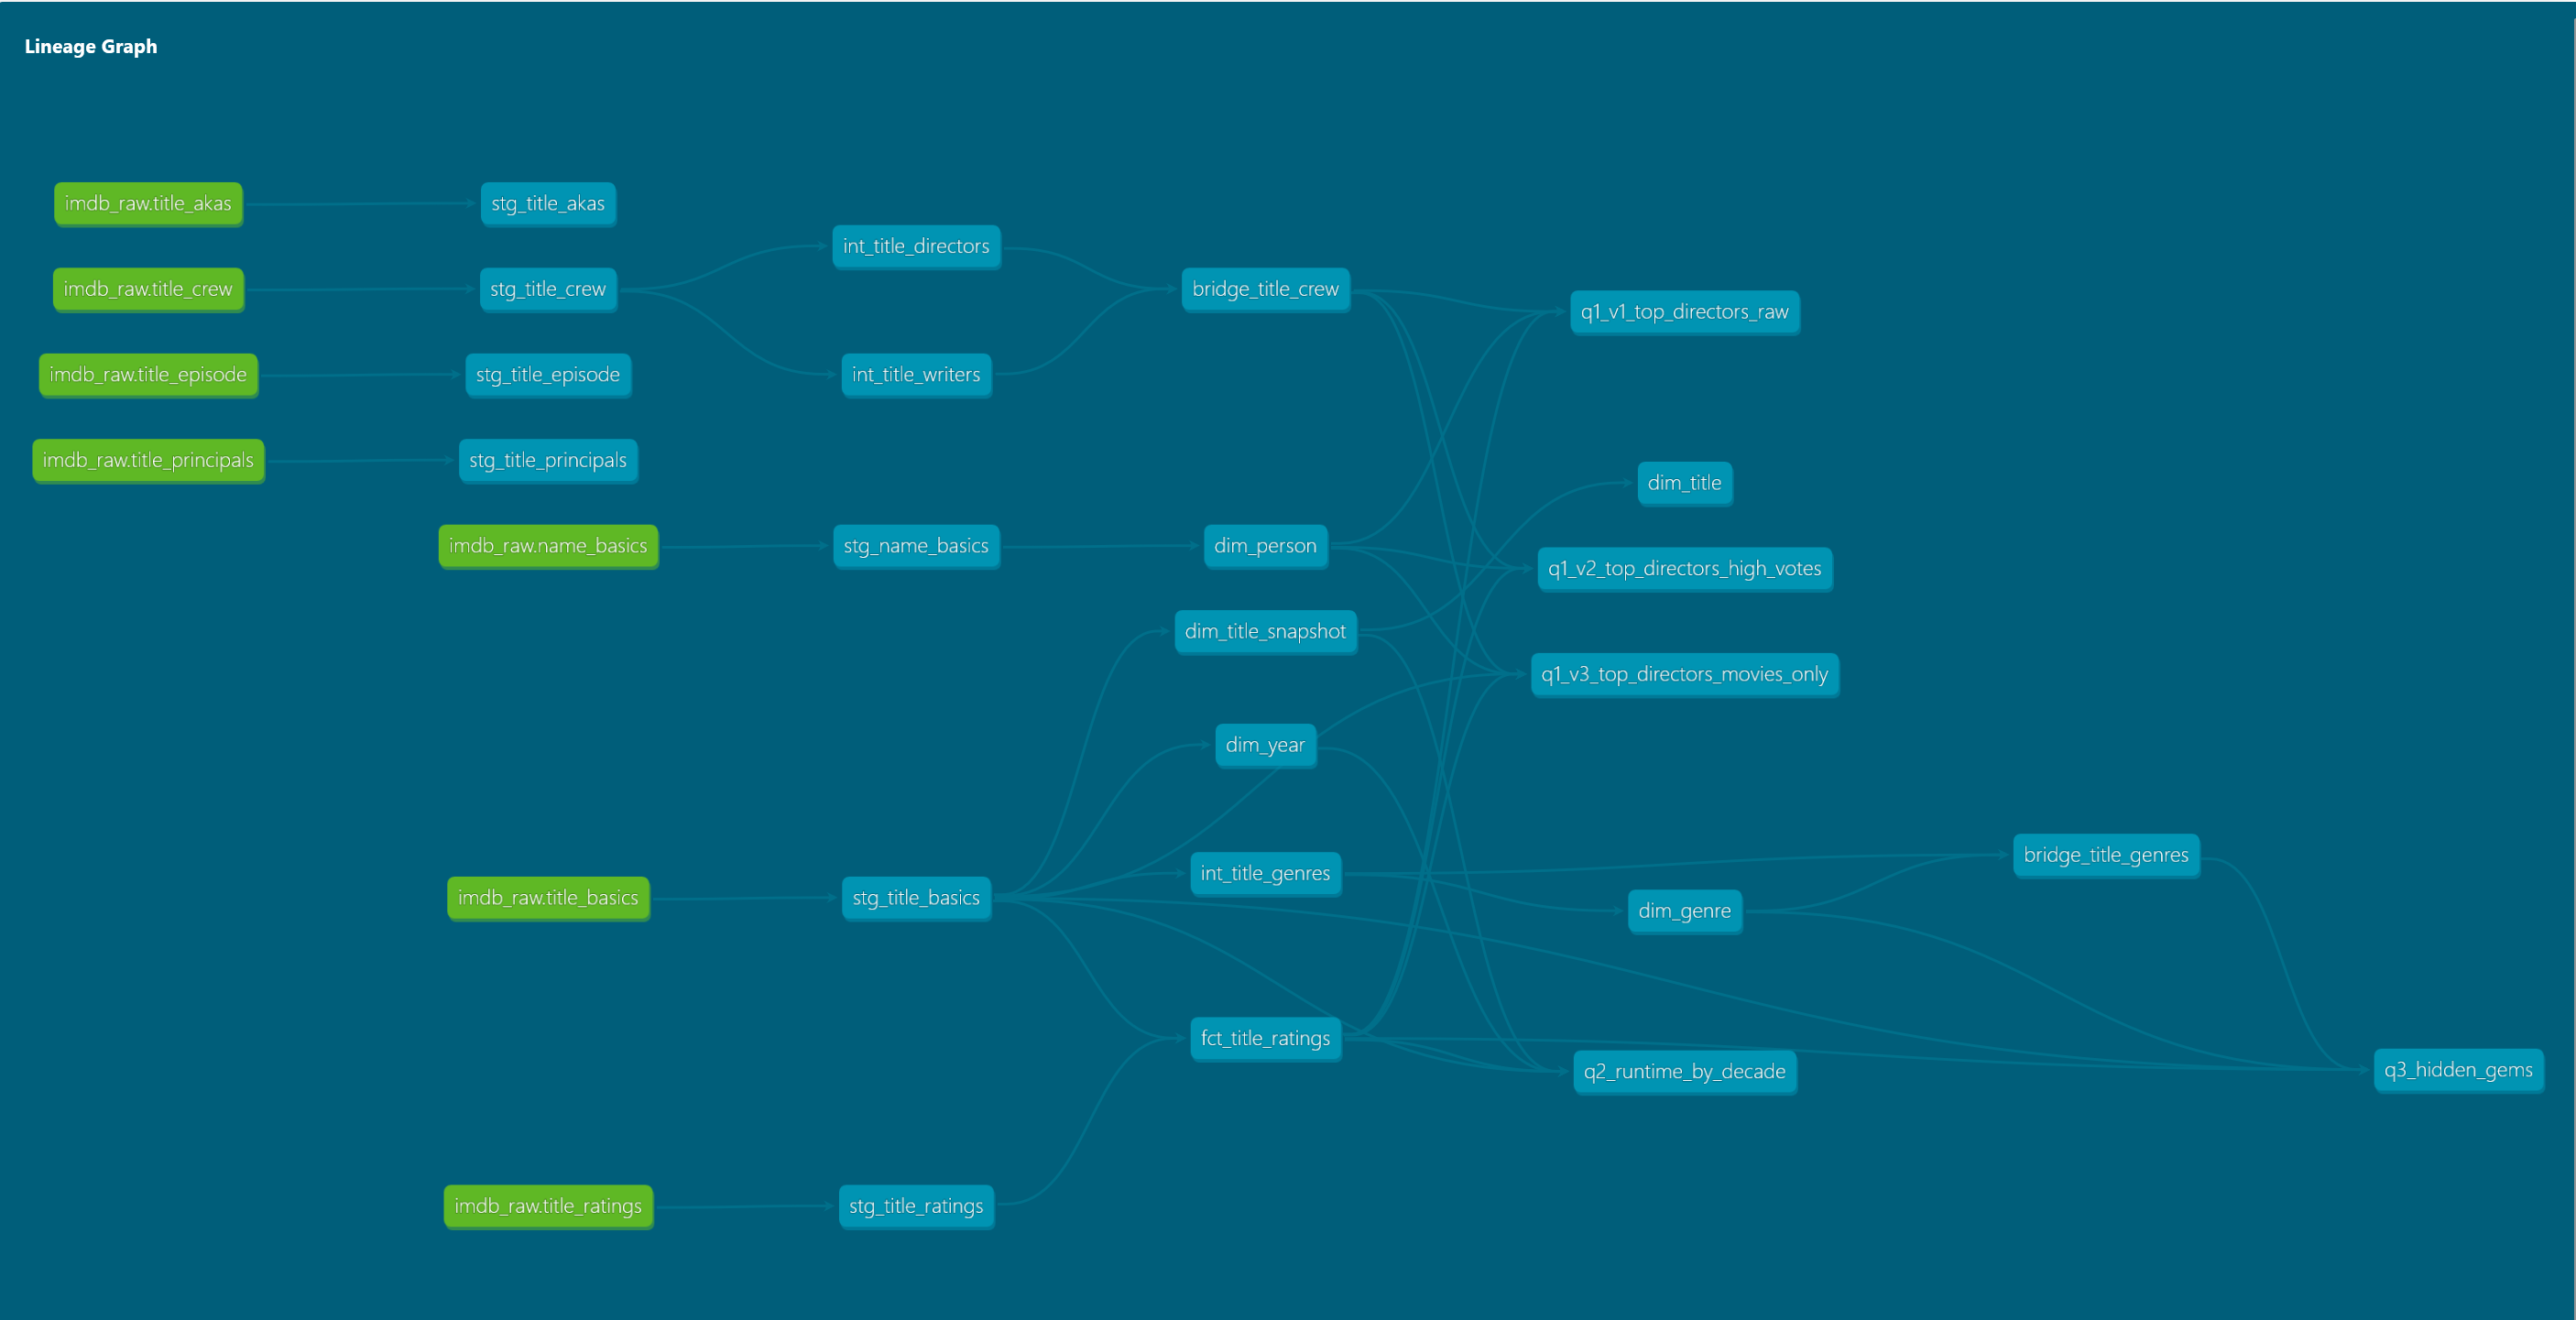
\includegraphics[width=1\textwidth]{dbt_lineage.png}
\caption{dbt docs lineage graph showing the transformation flow}
\label{fig:dbt_lineage}
\end{figure}

\subsection{Implemented Data Tests}

\begin{itemize}
    \item \textbf{Primary Key Tests (\texttt{unique} and \texttt{not\_null}):} Applied to the primary keys of all staging and mart tables (e.g., \texttt{title\_id} in \texttt{dim\_title\_snapshot} and \texttt{fct\_title\_ratings}).
    \\ \textit{Reason:} Ensures that no duplicate records exist and that foundational identifiers are never missing.

    \item \textbf{Referential Integrity Tests (\texttt{relationships}):} Applied to the foreign keys in the fact and bridge tables, validating that every \texttt{title\_id}, \texttt{name\_id}, or \texttt{year\_id} explicitly exists in their respective dimension tables.
    \\ \textit{Reason:} Prevents orphaned records in the data warehouse and guarantees that analytical aggregations group correctly across dimensions.

    \item \textbf{Domain Rule: Rating Range (Custom Test):} A custom SQL test applied to \texttt{average\_rating} in the fact table, ensuring values fall strictly between 0.0 and 10.0.
    \\ \textit{Reason:} Enforces raw business logic; IMDb ratings cannot mathematically exceed 10 or drop below 0. Values outside this range indicate data corruption.

    \item \textbf{Domain Rule: Valid Release Year (Custom SQL):} A custom validation applied to the \texttt{dim\_year} / \texttt{startYear} logic ensuring the year is not set in the distant future.
    \\ \textit{Reason:} Prevents manual data entry typos in the source system from corrupting time-based historical analyses.

    \item \textbf{Expected Failures / Warning Tests (\texttt{severity: warn}):} Applied to nullable descriptive fields, such as missing \texttt{runtimeMinutes} for obscure indie titles, or missing \texttt{genres}.
    \\ \textit{Reason:} Some titles in the raw dataset legitimately lack full metadata. Failing the pipeline on these rows would unnecessarily discard valid rating facts, so a warning is logged instead to maintain pipeline resilience.
\end{itemize}

\section{How to Run}
To ensure reproducibility, the pipeline can be executed either fully automated via Docker and Apache Airflow, or manually via a local terminal. Both methods require starting from a clean DuckDB environment.

\subsection{Prerequisites: Getting the Raw Data}
Before executing the pipeline, the raw datasets must be acquired:
\begin{enumerate}
    \item Navigate to the official IMDb Datasets page (\url{https://datasets.imdbws.com/}).
    \item Download the following 7 compressed files (\texttt{.tsv.gz}): \texttt{name.basics}, \texttt{title.akas}, \texttt{title.basics}, \texttt{title.crew}, \texttt{title.episode}, \texttt{title.principals}, and \texttt{title.ratings}.
    \item Place all downloaded files directly into the \texttt{data/} folder in the project root.
\end{enumerate}

\subsection{Execution via Airflow (Docker)}
This is the recommended approach for full orchestration:
\begin{enumerate}
    \item \textbf{Configure Environment:} Copy the environment variables template to create the local configuration file.
    \begin{itemize}
        \item \textit{Linux / macOS / WSL:} \texttt{cp .env.example .env}
        \item \textit{Windows (CMD / PowerShell):} \texttt{copy .env.example .env}
    \end{itemize}
    \item \textbf{Clean the Environment:} Delete any existing \texttt{warehouse/imdb.duckdb} file to ensure a clean state.
    \item \textbf{Start Containers:} Spin up the Docker containers by running: \texttt{docker compose up -d}.
    \item \textbf{Trigger DAG:} Access the Airflow UI at \texttt{http://localhost:8084} (credentials: \texttt{admin} / \texttt{admin}). Unpause and manually trigger the \texttt{imdb\_pipeline} DAG to execute all stages sequentially.
\end{enumerate}

\subsection{Local Execution (Without Airflow)}
To run the pipeline directly in a local terminal for debugging or testing:
\begin{enumerate}
    \item \textbf{Set up the Python Environment:} Create and activate a virtual environment, then install dependencies:
    \begin{verbatim}
python -m venv .venv
source .venv/bin/activate
pip install -r airflow/requirements.txt
pip install duckdb pandas matplotlib seaborn
    \end{verbatim}
    \item \textbf{Clean the State:} Delete the \texttt{warehouse/imdb.duckdb} file.
    \item \textbf{Extract \& Load:} Run the extraction script to build the DuckDB Bronze layer: \texttt{python scripts/load\_imdb.py}.
    \item \textbf{Transform \& Test:} Execute the transformation and testing layers via dbt in the root directory by running: \texttt{dbt build}.
\end{enumerate}

\section{Answers to the Deliverable Questions}

\subsection{Q1: Top 10 Directors}
\textbf{Question:} Who are the top 10 directors by average rating, restricted to those with 5+ titles and 1,000+ combined votes?

\noindent\textbf{Model/Query Used:} \texttt{q1\_v3\_top\_directors\_movies\_only.sql}

\noindent\textbf{Result:} After filtering specifically for feature films, established Hollywood directors such as Christopher Nolan and Quentin Tarantino emerged at the top of the list.

\noindent\textbf{Interpretation:} Filtering strictly for \texttt{title\_type = 'movie'} is critical to eliminate "data skew," as TV episodes and obscure short films inherently receive much higher baseline ratings from niche audiences than mainstream cinema.


\subsection{Q2: Movie Runtime Evolution}
\textbf{Question:} Has the average movie runtime changed by decade, and does runtime correlate with rating?

\noindent\textbf{Model/Query Used:} \texttt{q2\_runtime\_by\_decade.sql}

\noindent\textbf{Result:} The average feature film runtime has remained incredibly stable at around 94--97 minutes since the 1980s; however, the correlation between longer runtimes and higher ratings dropped from a strong positive in the 1940s--1970s to near zero in the modern era.

\noindent\textbf{Interpretation:} While the long epics of the "Golden Age" were treated as prestigious cultural events that audiences deeply appreciated, modern audiences do not systematically reward a movie with higher ratings simply because it has a longer runtime.


\subsection{Q3: Hidden Gems vs. Overrated Titles}
\textbf{Question:} Which genres have the highest ratio of "hidden gems" (high rating, low vote count) versus "overrated" titles (low rating, high vote count)?

\noindent\textbf{Model/Query Used:} \texttt{q3\_hidden\_gems.sql}

\noindent\textbf{Result:} Documentary, History, and War genres have the highest ratio of hidden gems, whereas Sci-Fi, Horror, and Action genres have the worst ratios, making them the most overrated.

\noindent\textbf{Interpretation:} Niche genres attract passionate audiences who consistently rate them highly, whereas mass-market blockbusters attract huge vote counts due to marketing but frequently fail to deliver on quality, resulting in mediocre ratings.

\section{Challenges and Lessons Learned}

\begin{enumerate}
    \item \textbf{Handling IMDb's Custom Null Representations (\textbackslash N)} \\
    A significant data quality issue arose during the transformation phase due to IMDb's formatting choices. The raw TSV files use the literal string "\textbackslash N" to represent missing data. Attempting to cast numeric columns (such as \texttt{runtimeMinutes} or \texttt{startYear} to integer types) directly in DuckDB or dbt caused the pipeline to crash with type mismatch errors. \\
    \textbf{Resolution:} By wrapping the affected columns in a \texttt{NULLIF(column\_name, '\textbackslash N')} function before applying the \texttt{CAST()} operation, the pipeline safely converts these string literals into true SQL \texttt{NULL} values, preventing runtime failures.

    \item \textbf{Data Skew and "Noise" in Analytical Aggregations} \\
    When initially calculating the top directors by average rating, the results were heavily skewed. Directors of obscure short films or highly-rated television anime episodes consistently ranked above established cinema directors due to the inherently different voting behaviors across media types. \\
    \textbf{Resolution:} I had to refine the business logic in the final analytical queries. By explicitly joining the \texttt{staging} metadata and enforcing a strict \texttt{title\_type = 'movie'} filter, the noise was successfully eliminated, yielding accurate insights.

   \item \textbf{Challenge: Schema Inconsistencies During Parquet Migration} \\
    When migrating the orchestration to Airflow, the extraction architecture was simultaneously updated to convert the raw TSV files into Parquet format before loading them into DuckDB. Following this change, downstream dbt tasks (such as \texttt{dbt\_run\_staging} and \texttt{dbt\_snapshot}) began failing intermittently, as seen in the Airflow Grid View. These seemingly random crashes occurred because DuckDB infers schemas differently from Parquet files compared to raw TSV reads, exposing new type-casting inconsistencies that the initial dbt models were not prepared for. \\
    \textbf{Resolution:} The pipeline was stabilized by enforcing much stricter SQL \texttt{CAST} operations directly within the dbt \texttt{staging} layer. Instead of altering the ingestion script, the staging models were updated to rigorously cast and handle the inferred Parquet data types, ensuring all downstream models received a uniform and predictable schema.
\end{enumerate}

\end{document}
